\chapter{Survey of Anchor Node Placements}

\section{Measuring Location Error}
Before searching for the best anchor node placement we must first define what \emph{best} means, in terms of location error.  First of all, location error is measured as a factor of radio radius (or range).  Since this study addresses range-free networks, and thus relies solely on network connectivity, the actual units of distance do not matter for general study.  What is important is how many other nodes in the network fall within the radio range of a given node.  The average numbers of nodes within range of a each node is known as connectivity.

Every network has its own application requirements, and thus there are many options for what statistics to examine for accessing the quality of locations.  The simplest criteria are to look at the mean and maximum location error across all nodes in the network.  For the most part, this is the basis for the results in this study.  However, this assumes that all nodes in the network must be used in the final results.  If the network designers know which nodes have poor locations, they may wish to exclude these nodes from the final results.  Therefore, if the economics of the network deployment allow, it may be beneficial to look at the best, for example, 80\% of nodes in the network.  In practice, the designers do not know which nodes to exclude, so this study also attempts to identify the worst areas of a network for location accuracy, depending on the anchor node placement.  

\section{Insignificant Factors}
A number of hypotheses of anchor node placement were attempted, but showed no significant correlation to location error.  The following is a summary of what some may assume matter, but in reality does not.

\subsection{Number of Neighbors}
\begin{figure}
  \centering
      \subfloat[The Data]{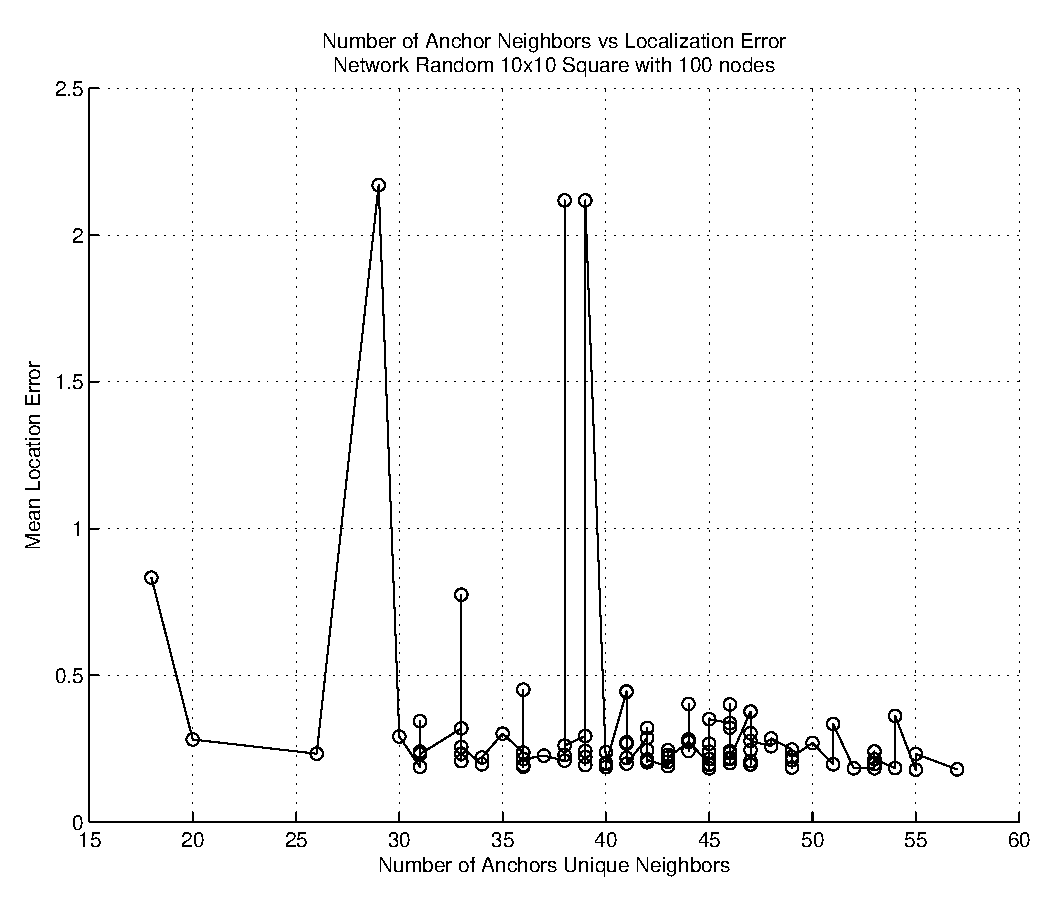
\includegraphics[width=0.5\textwidth]{AnchorNeighborsVsError-Random-10x10-Square-with-100-nodes-Radius2.5-to-2.5.eps}}
    \subfloat[The Network]{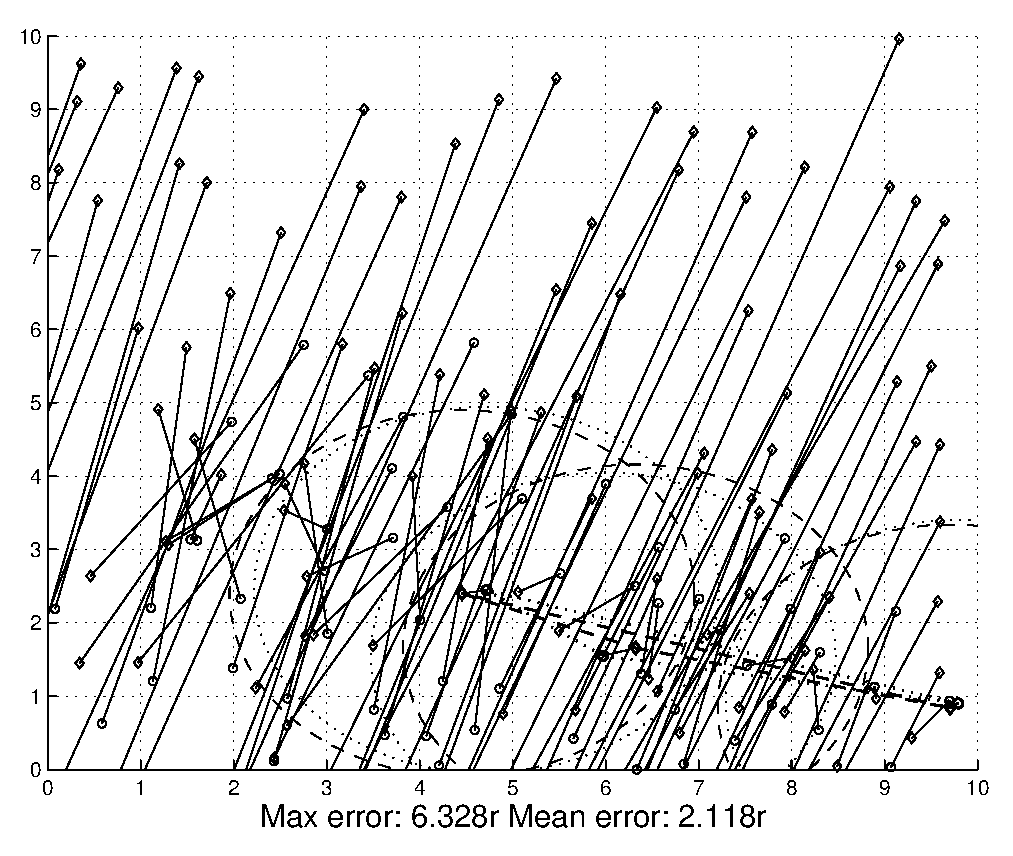
\includegraphics[width=0.5\textwidth]{NetDiff-R2.5-Rank98-AnchorSet12-.eps}}
    \caption{Number of Anchor Neighbors vs Location Error}
    \label{fig:Neighbors1}
\end{figure}

One theory is that the nodes that are one-hop away from an anchor would have better location accuracy.  As shown in Figure ~\ref{fig:Neighbors1}, the effect of the number of neighbors is random.  Figure ~\ref{fig:Neighbors1Network} shows the best of the chosen anchor sets, in terms of mean node location error and the difference between the actual and calculated locations.  Further, the three nodes with the worst locations are within one hop of an anchor.  In the end, having more neighbors means that the error of the anchor node itself has a better calculated location accuracy as show in TODO, but this does not translate into better network-wide accuracy.


\subsection{Anchors Farther Apart}


\section{Significant Factors}

\subsection{Height of Triangle Formed by Anchors}

\begin{figure}
  \centering
    \subfloat[Height]{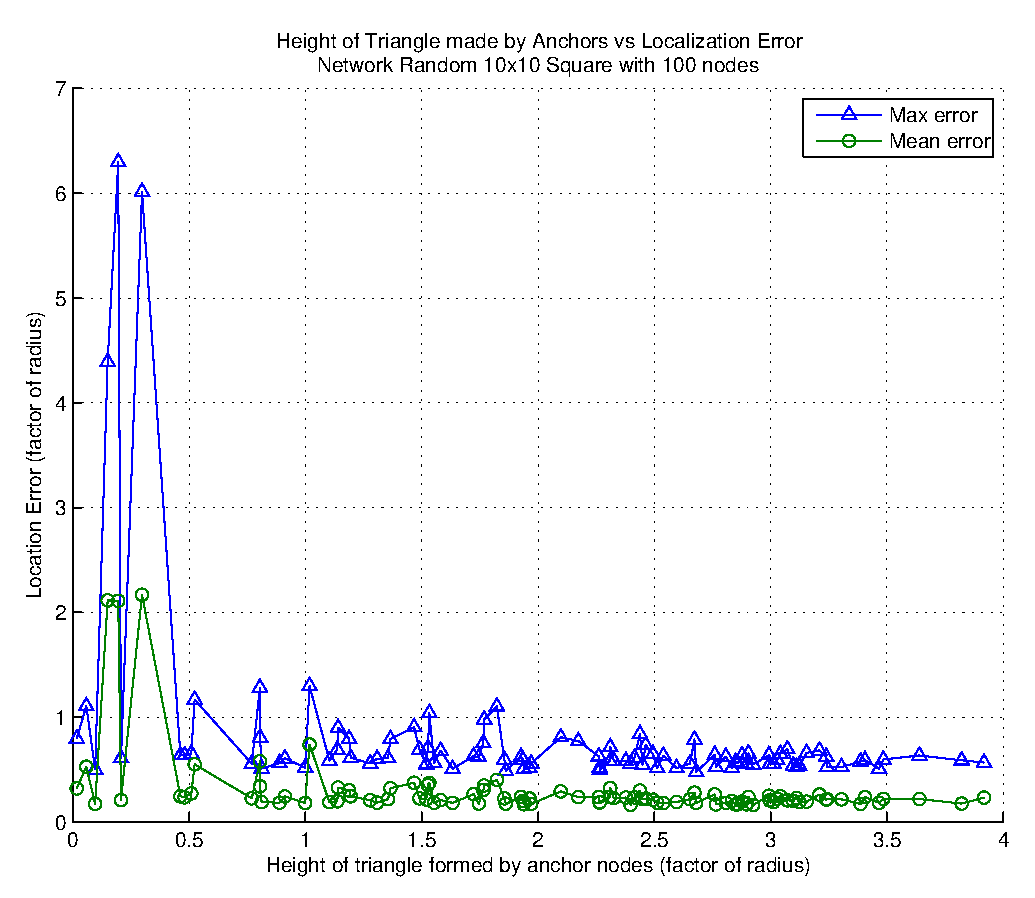
\includegraphics[width=0.5\textwidth]{AnchorTriangleHeightVsError-Random-10x10-Square-with-100-nodes.eps}}
    \subfloat[Area]{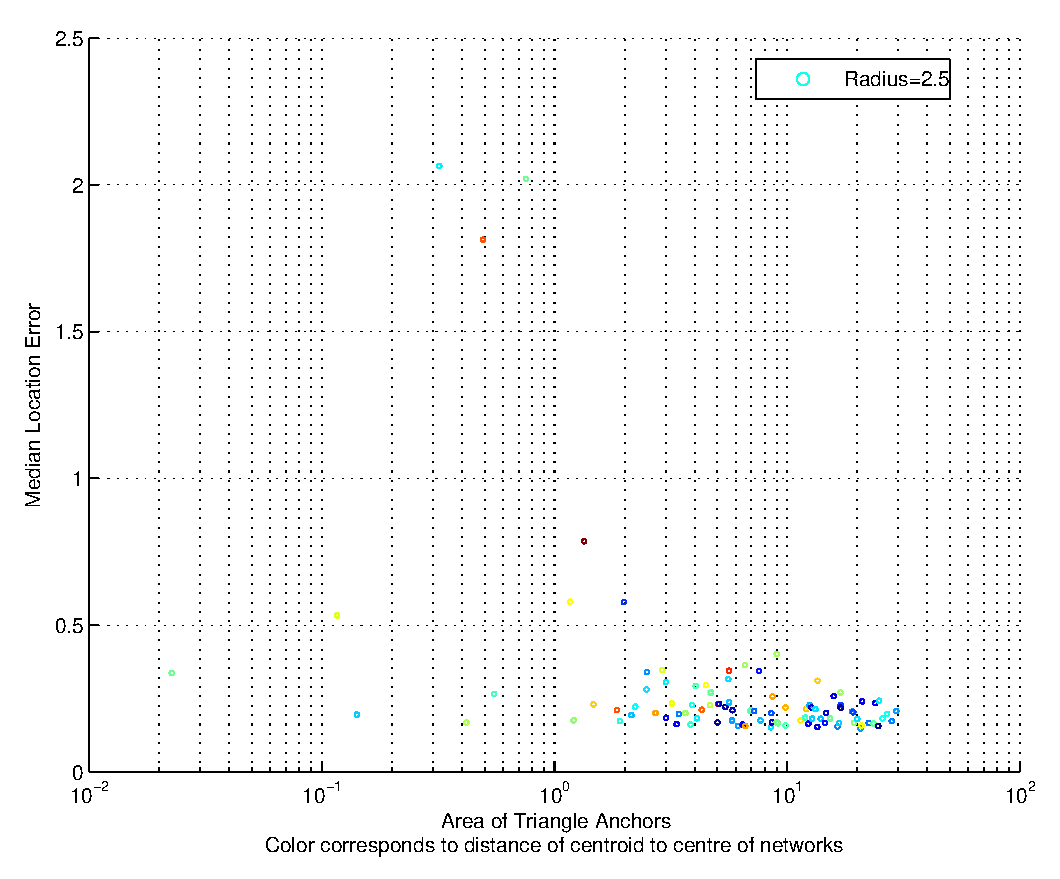
\includegraphics[width=0.5\textwidth]{AnchorTriangleAreaVsError-Random-10x10-Square-with-100-nodes.eps}}
    \label{fig:Triangle1}
\end{figure}

